\documentclass[usenatbib]{mnras}
\usepackage{graphicx,xspace}
\newcommand{\Gaia}{\textit{Gaia}\xspace}
\newcommand{\HST}{\textit{HST}\xspace}
\newcommand{\kms}{km\:s$^{-1}$\xspace}
\newcommand{\masyr}{mas\:yr$^{-1}$\xspace}

\begin{document}

\clearpage\begin{figure*}
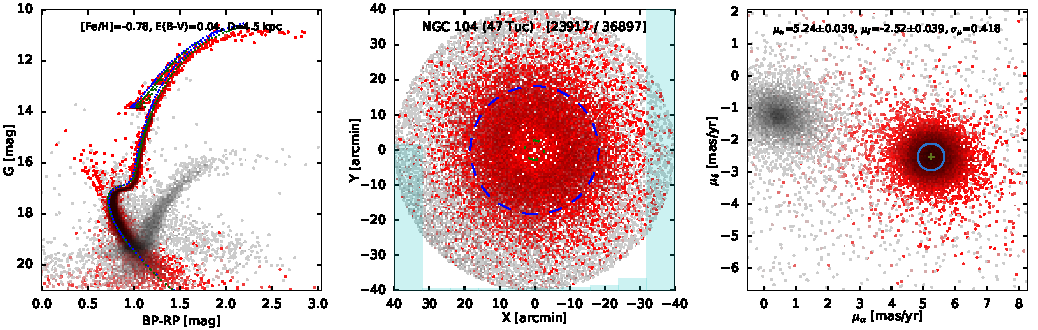
\includegraphics{figs/NGC_104_47Tuc.pdf}
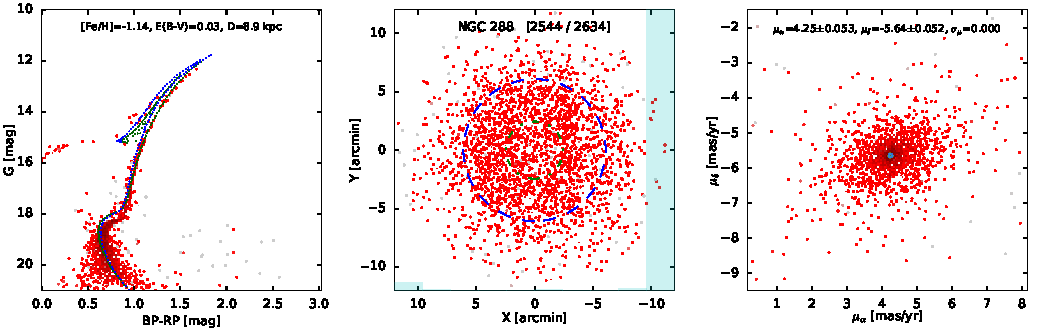
\includegraphics{figs/NGC_288.pdf}
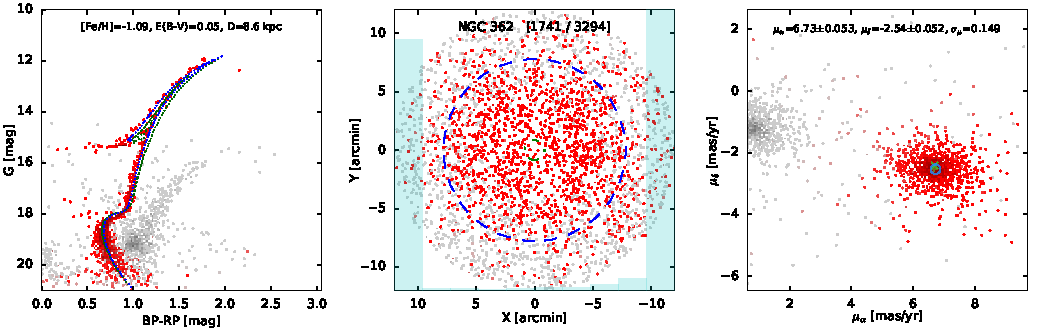
\includegraphics{figs/NGC_362.pdf}
\caption{
Colour--magnitude diagrams (left column), spatial distribution (middle column) and PM distribution (right column) of stars in individual clusters.
Membership probability is marked by colour (red -- likely members, gray -- field stars); the number of members and the total number of stars in the sample is given in brackets.
Green crosses indicate likely member stars listed in other papers. 
Isochrone tracks for the assumed age, metallicity and distance are plotted in the left panel by blue dots (PARSEC, \citealt{Bressan2012}) and green dots (MIST, \citealt{Choi2016}), with extinction and reddening computed using the coefficients from Table~1 in \citet{Babusiaux2018}.
Cyan histogram in the central panel shows the distribution of membership probabilities $p$ in 10 bins (leftmost -- $p\le 10\%$, rightmost -- $p\ge 90\%$); a strongly bimodal distribution indicates a good separation of cluster and field stars in the PM space. Green dot-dashed circle shows the half-light radius from \citet{Baumgardt2019}, and blue dashed circle -- the scale radius $R_\mathrm{scale}$ of the Plummer profile of member stars in the filtered \Gaia catalogue, which is typically larger than the true half-light radius because the catalogue is incomplete in the central regions.
Blue ellipse in the right panel indicates the uncertainty on the mean PM, summed in quadrature with the internal PM dispersion $\sigma_\mu$. Green crosses indicate the mean PM measured by \HST, and pluses -- by \citet{Helmi2018}.\protect\\
The plots for all 150 clusters are presented as supplementary material.
\protect\\
\textit{(Continued on the next page)}
}
\end{figure*}

\clearpage\begin{figure*}
\contcaption{}
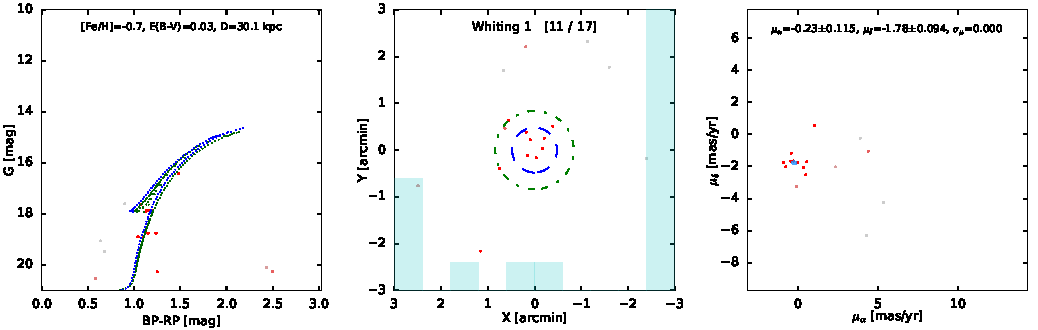
\includegraphics{figs/Whiting_1.pdf}
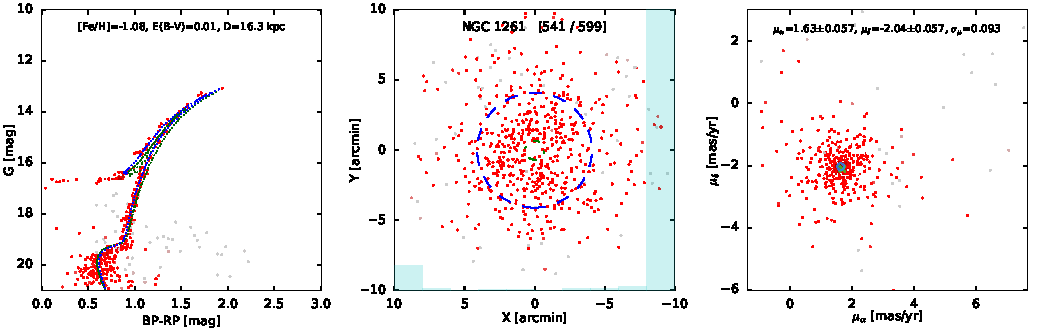
\includegraphics{figs/NGC_1261.pdf}
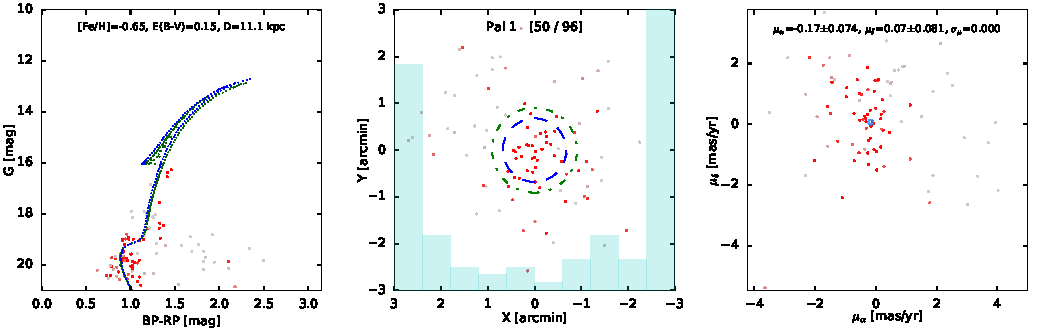
\includegraphics{figs/Pal_1.pdf}
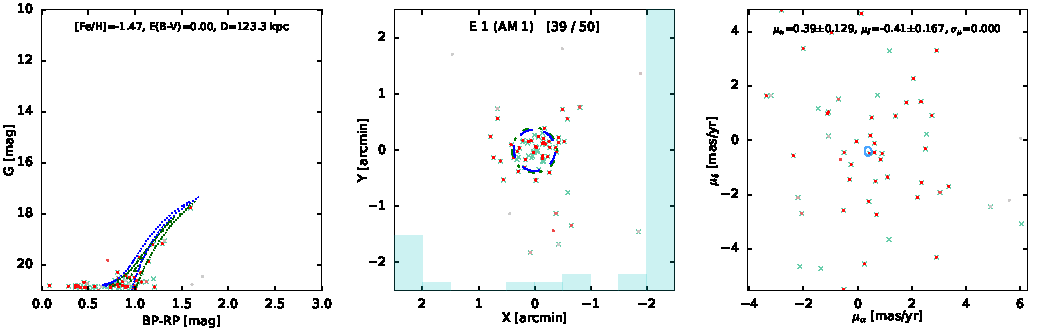
\includegraphics{figs/AM_1.pdf}
\end{figure*}

\clearpage\begin{figure*}
\contcaption{}
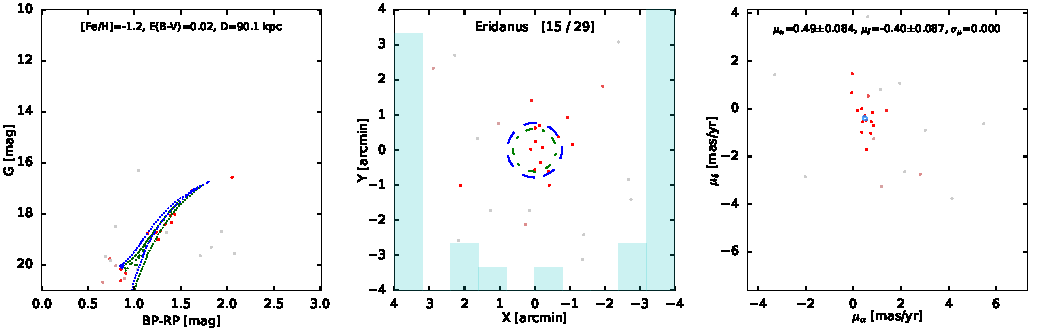
\includegraphics{figs/Eridanus.pdf}
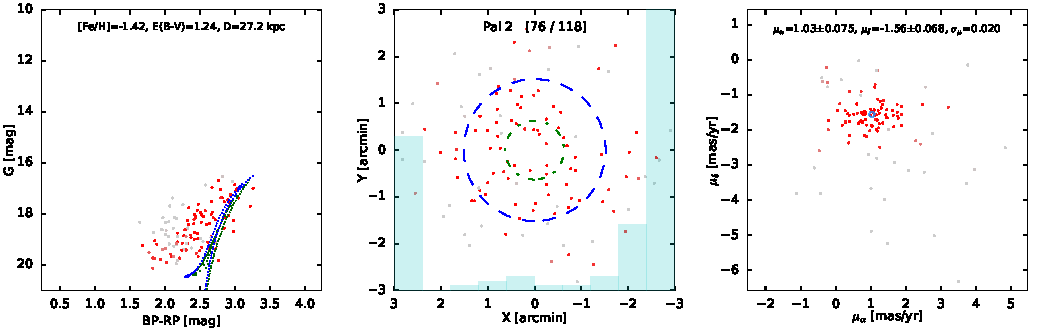
\includegraphics{figs/Pal_2.pdf}
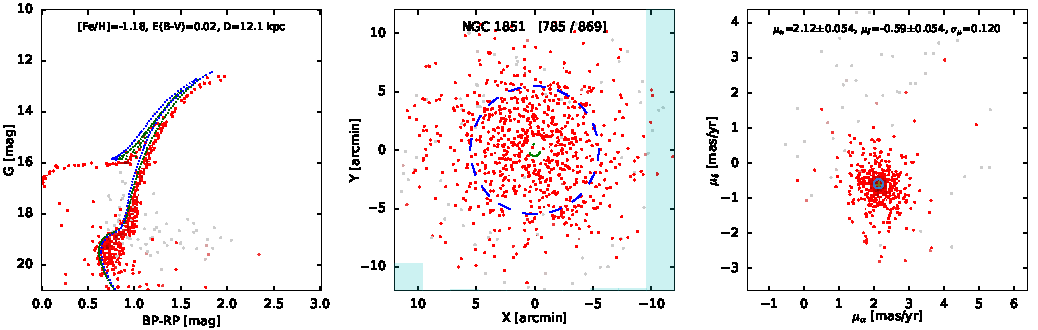
\includegraphics{figs/NGC_1851.pdf}
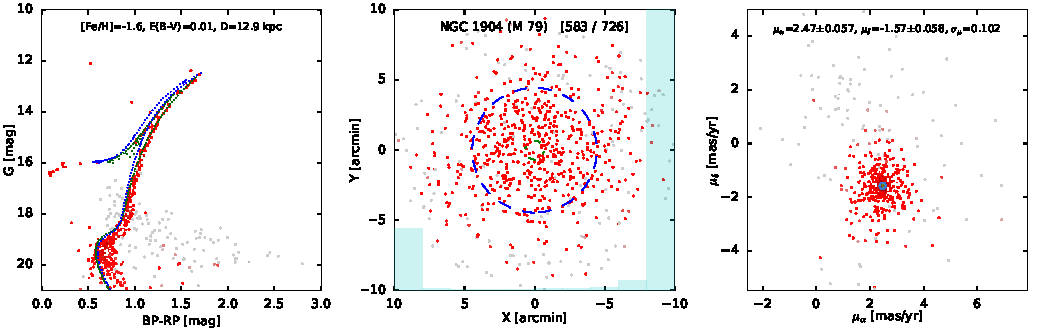
\includegraphics{figs/NGC_1904_M_79.pdf}
\end{figure*}

\clearpage\begin{figure*}
\contcaption{}
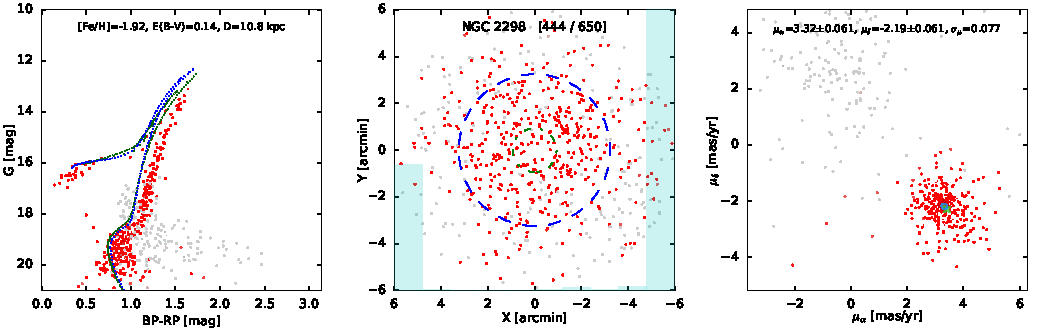
\includegraphics{figs/NGC_2298.pdf}
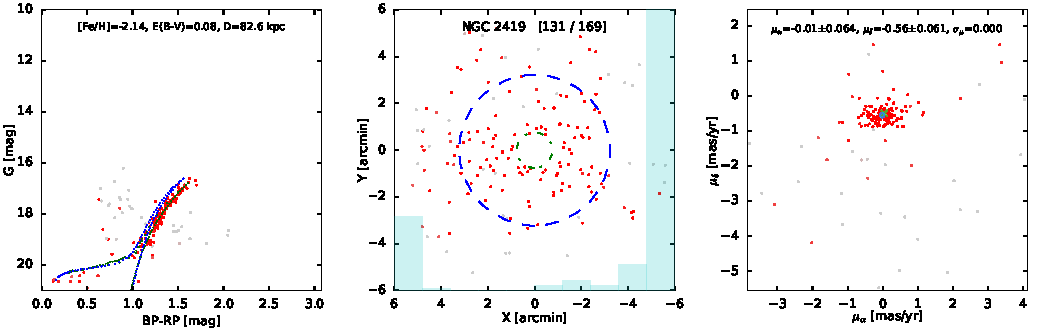
\includegraphics{figs/NGC_2419.pdf}
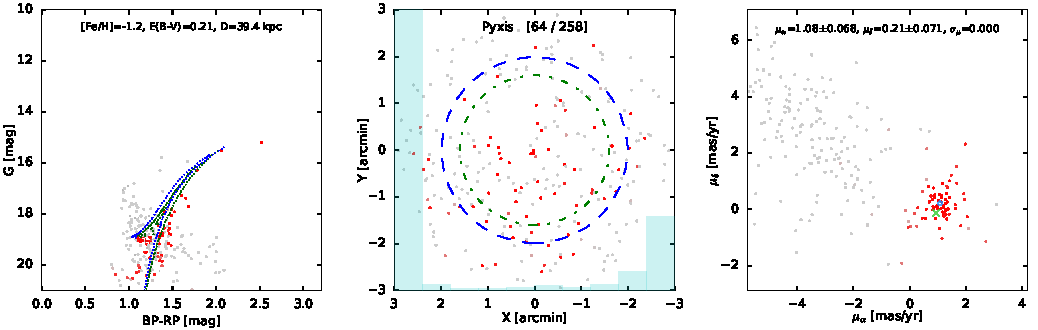
\includegraphics{figs/Pyxis.pdf}
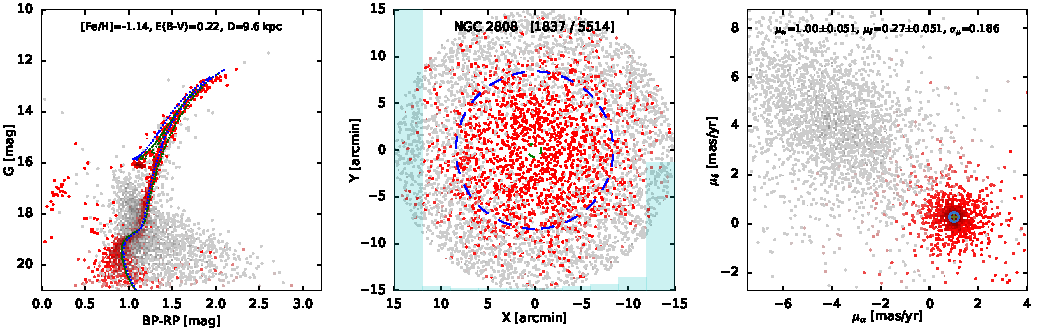
\includegraphics{figs/NGC_2808.pdf}
\end{figure*}

\clearpage\begin{figure*}
\contcaption{}
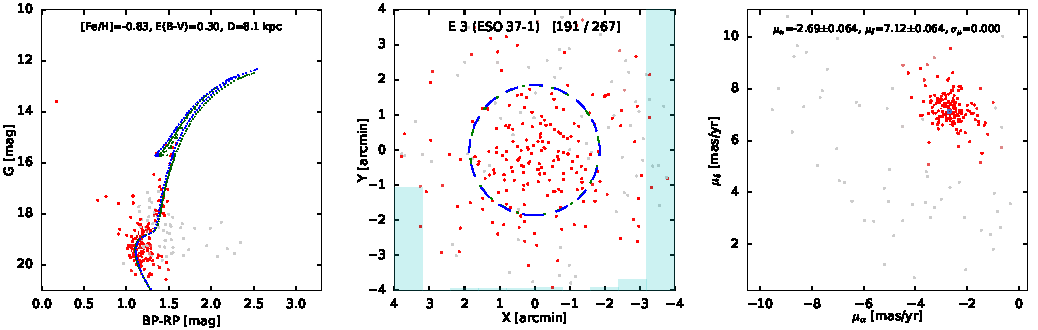
\includegraphics{figs/E_3.pdf}
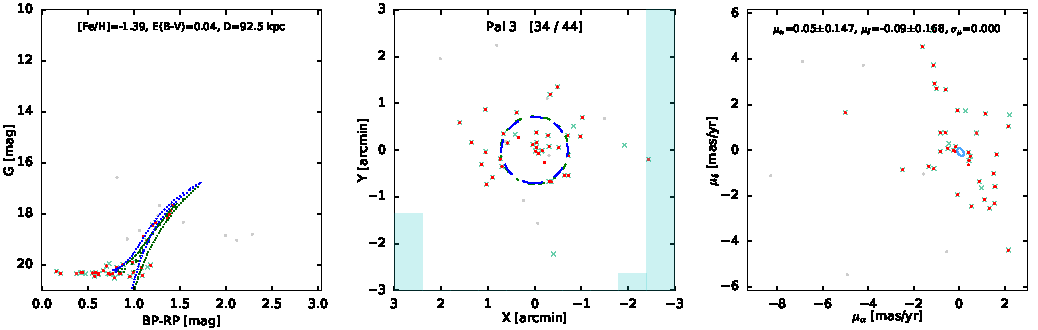
\includegraphics{figs/Pal_3.pdf}
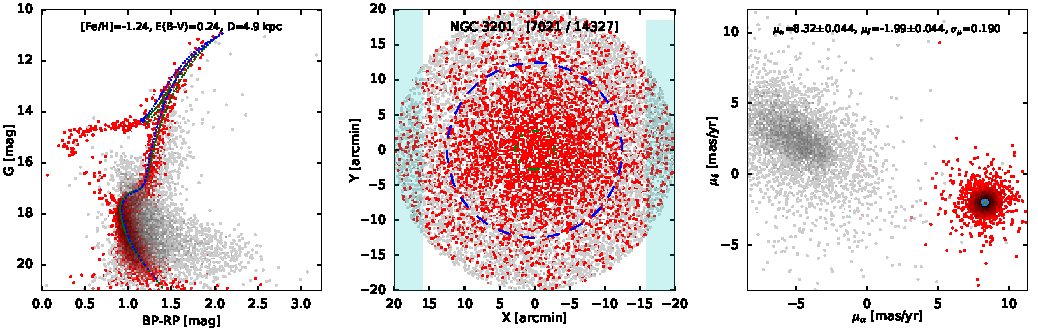
\includegraphics{figs/NGC_3201.pdf}
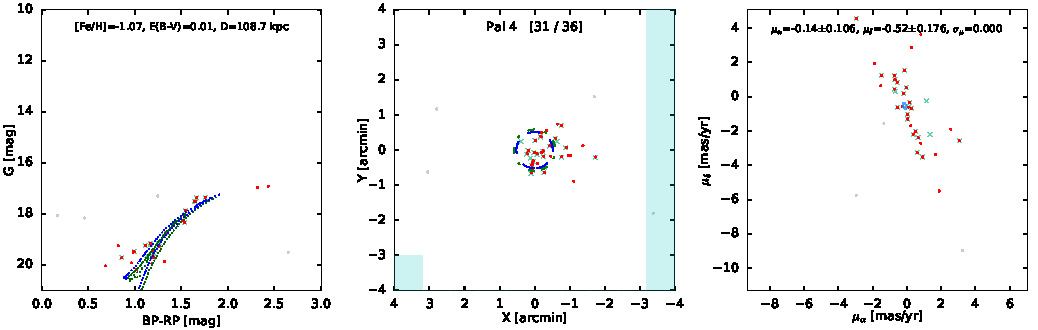
\includegraphics{figs/Pal_4.pdf}
\end{figure*}

\clearpage\begin{figure*}
\contcaption{}
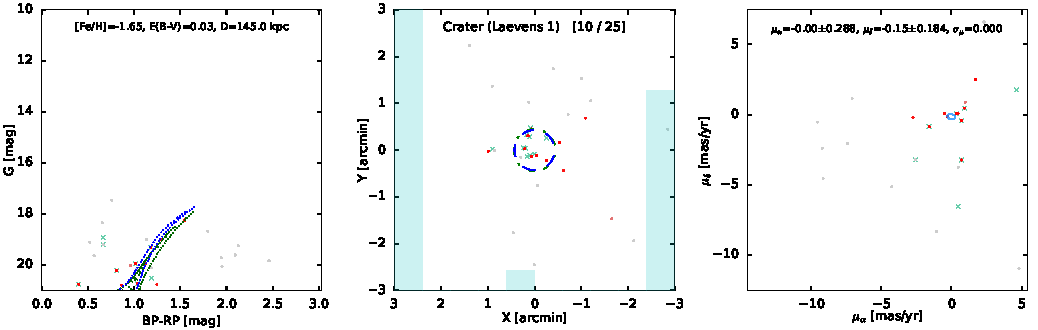
\includegraphics{figs/Crater.pdf}
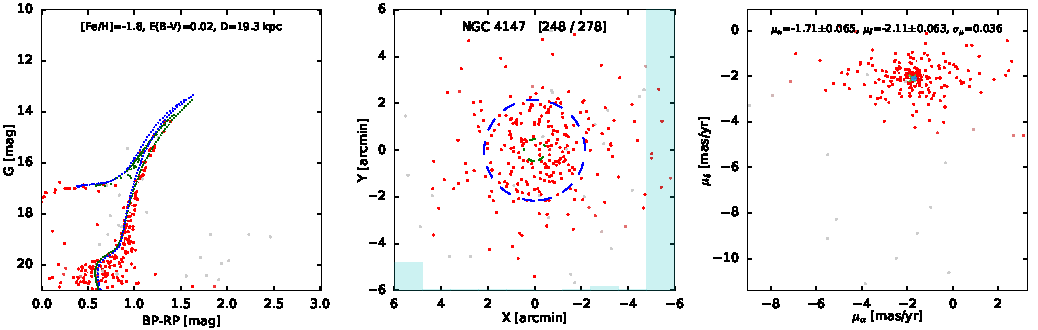
\includegraphics{figs/NGC_4147.pdf}
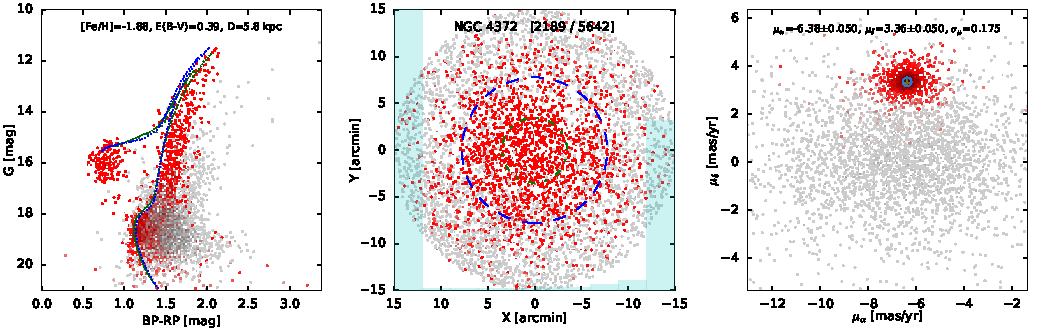
\includegraphics{figs/NGC_4372.pdf}
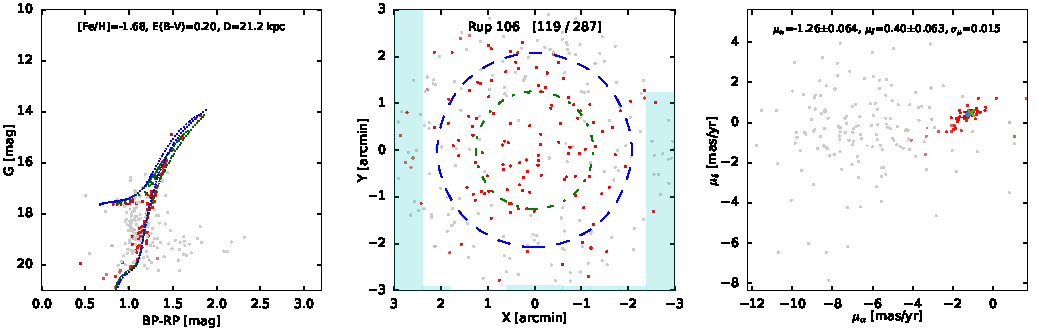
\includegraphics{figs/Rup_106.pdf}
\end{figure*}

\clearpage\begin{figure*}
\contcaption{}
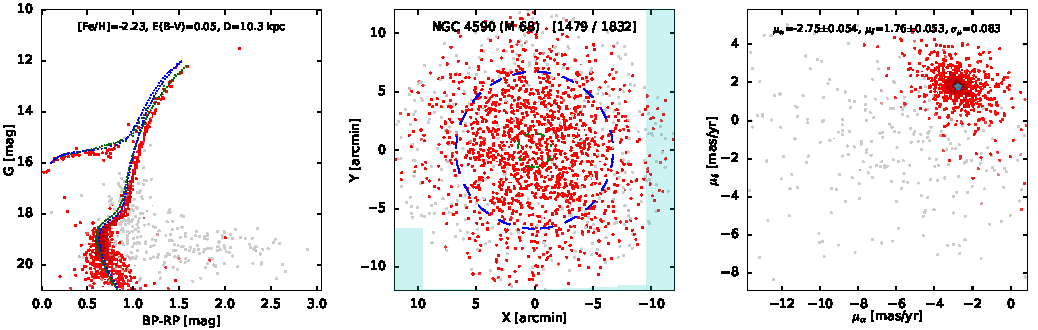
\includegraphics{figs/NGC_4590_M_68.pdf}
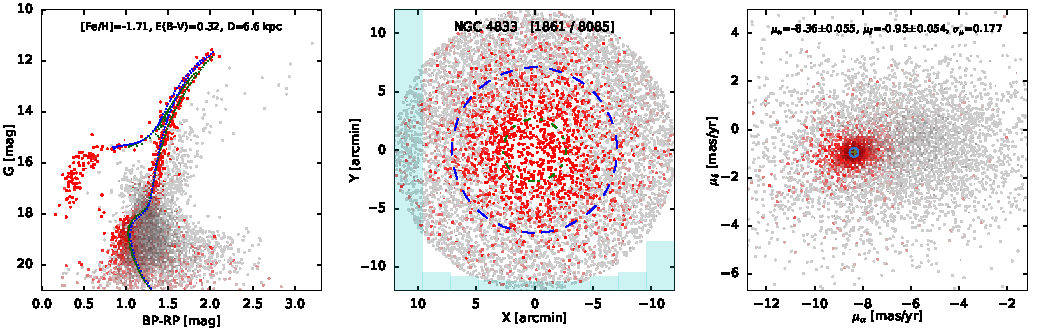
\includegraphics{figs/NGC_4833.pdf}
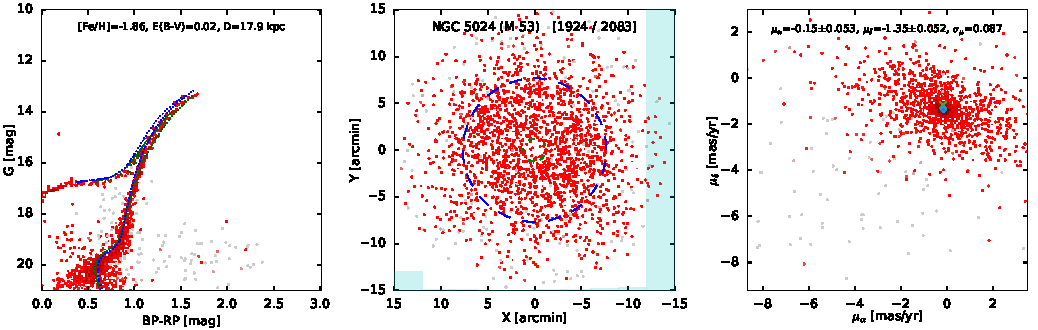
\includegraphics{figs/NGC_5024_M_53.pdf}
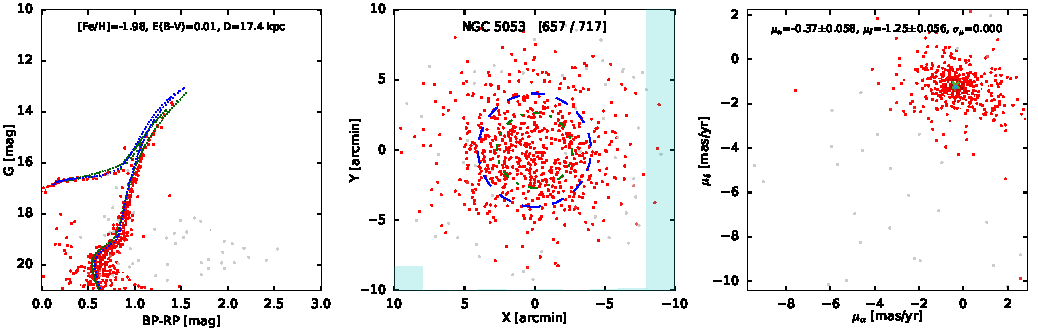
\includegraphics{figs/NGC_5053.pdf}
\end{figure*}

\clearpage\begin{figure*}
\contcaption{}
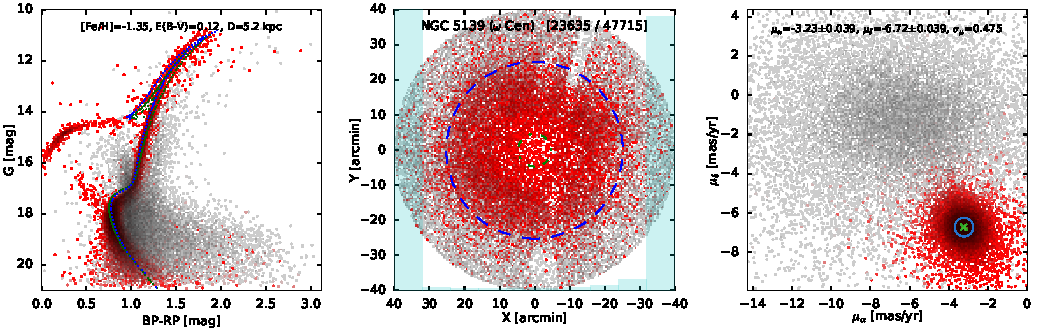
\includegraphics{figs/NGC_5139_oCen.pdf}
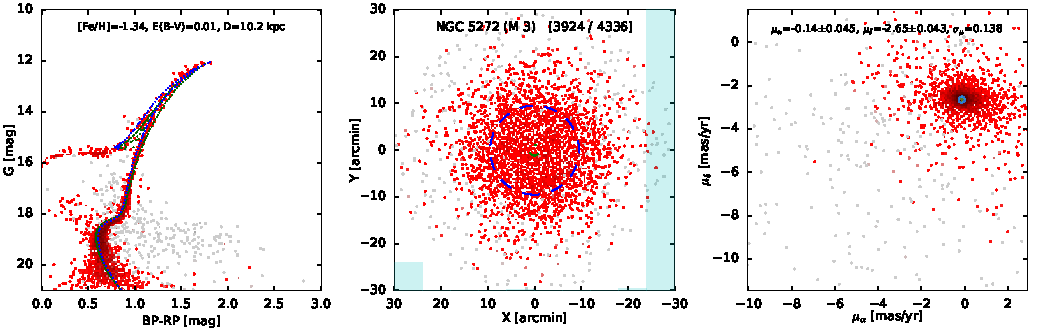
\includegraphics{figs/NGC_5272_M_3.pdf}
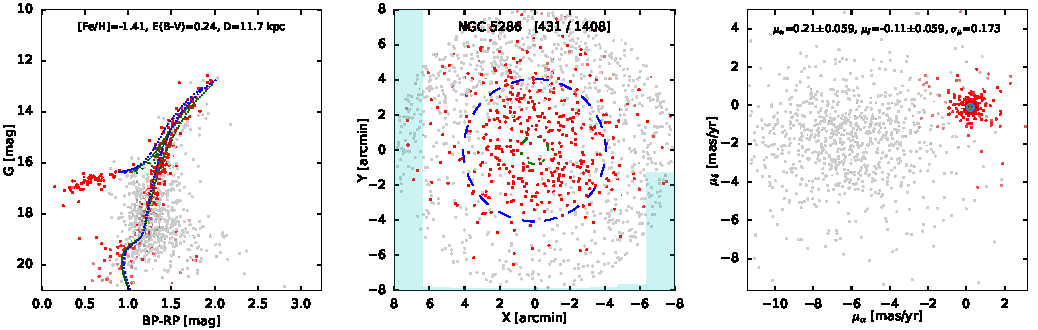
\includegraphics{figs/NGC_5286.pdf}
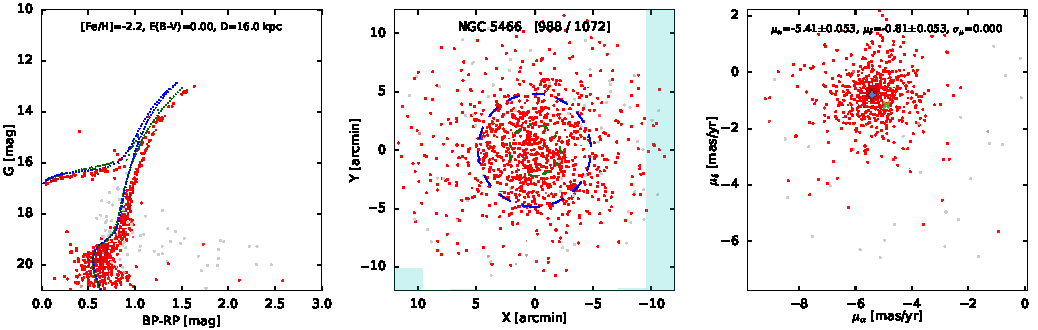
\includegraphics{figs/NGC_5466.pdf}
\end{figure*}

\clearpage\begin{figure*}
\contcaption{}
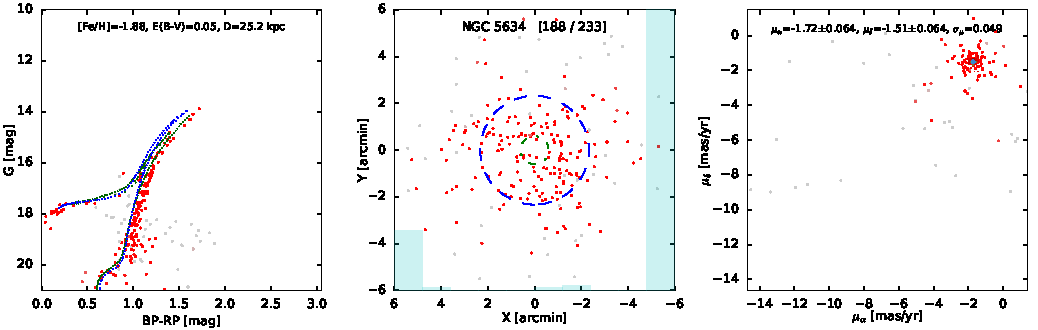
\includegraphics{figs/NGC_5634.pdf}
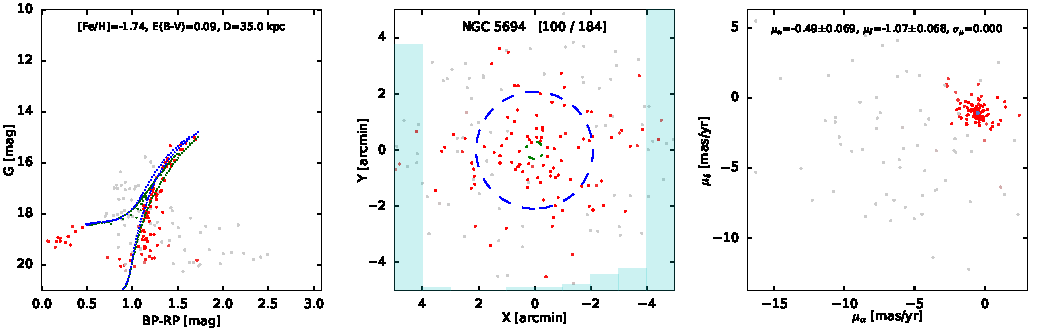
\includegraphics{figs/NGC_5694.pdf}
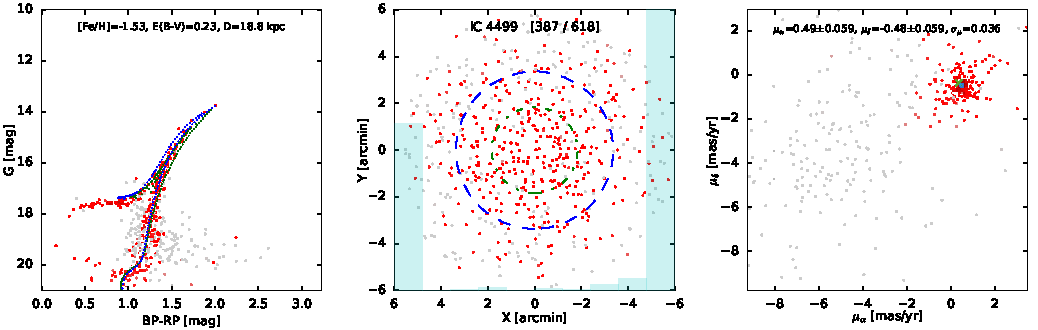
\includegraphics{figs/IC_4499.pdf}
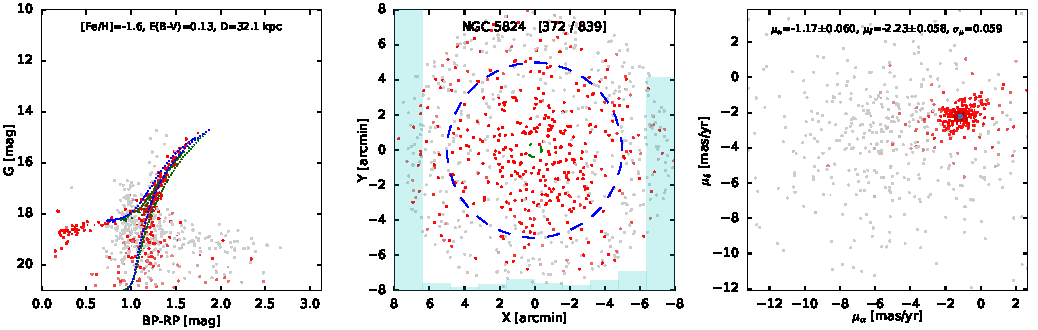
\includegraphics{figs/NGC_5824.pdf}
\end{figure*}

\clearpage\begin{figure*}
\contcaption{}
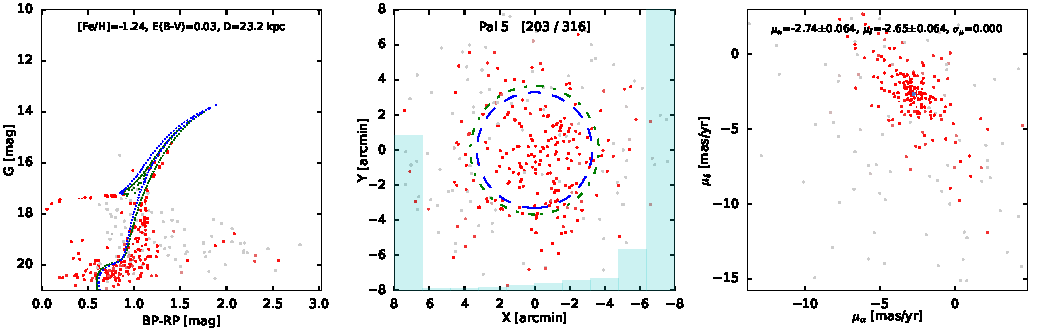
\includegraphics{figs/Pal_5.pdf}
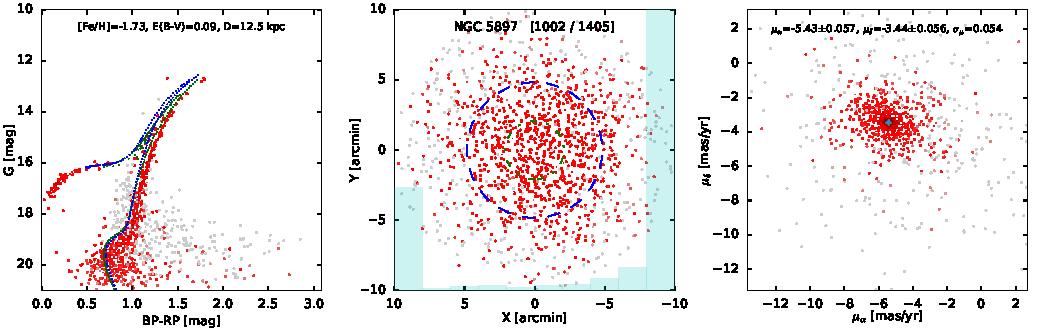
\includegraphics{figs/NGC_5897.pdf}
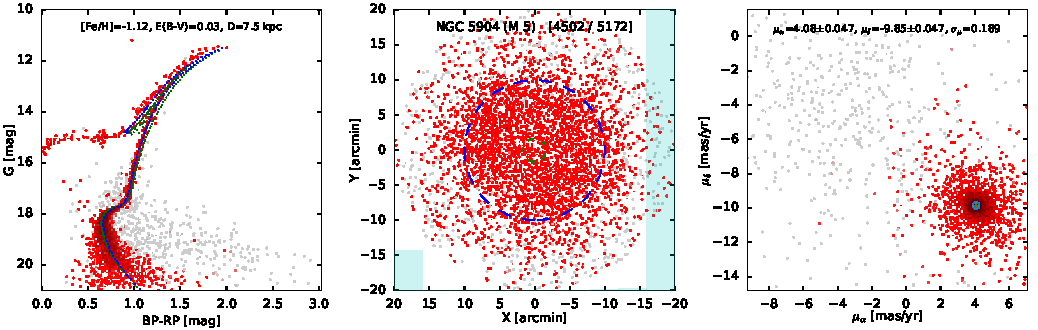
\includegraphics{figs/NGC_5904_M_5.pdf}
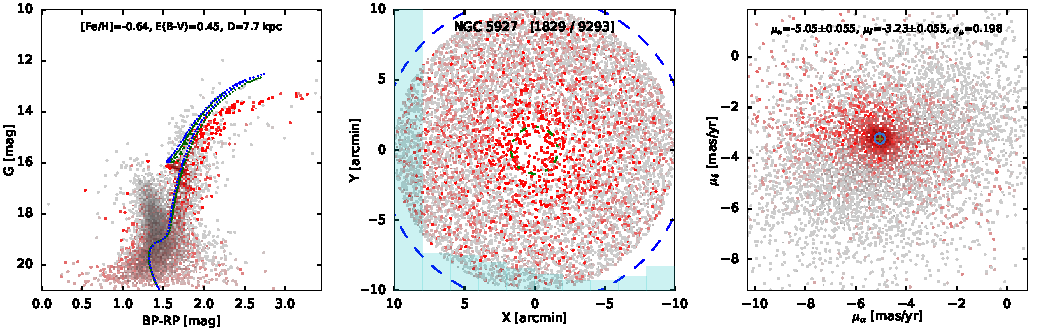
\includegraphics{figs/NGC_5927.pdf}
\end{figure*}

\clearpage\begin{figure*}
\contcaption{}
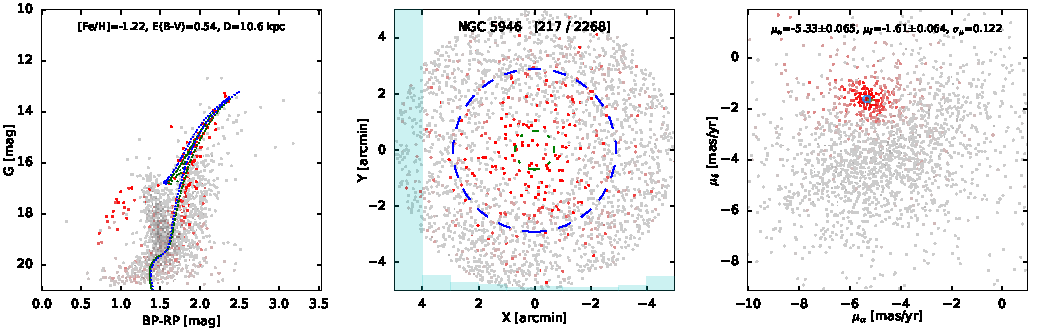
\includegraphics{figs/NGC_5946.pdf}
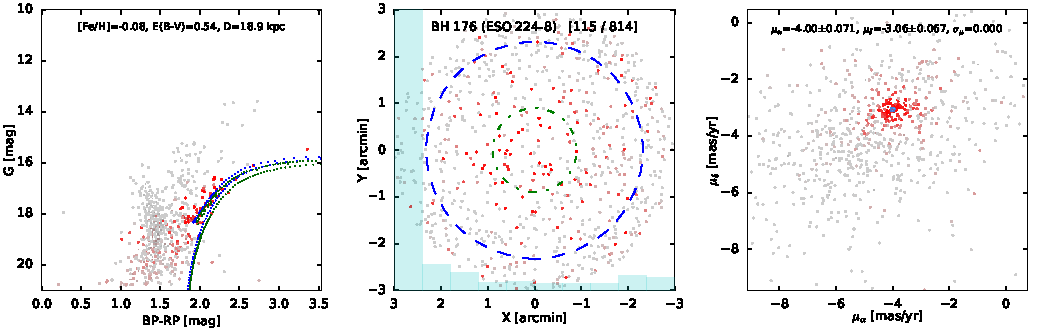
\includegraphics{figs/BH_176.pdf}
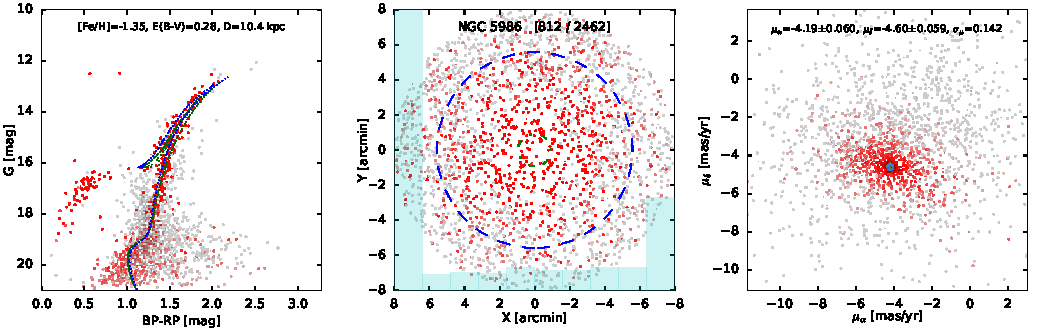
\includegraphics{figs/NGC_5986.pdf}
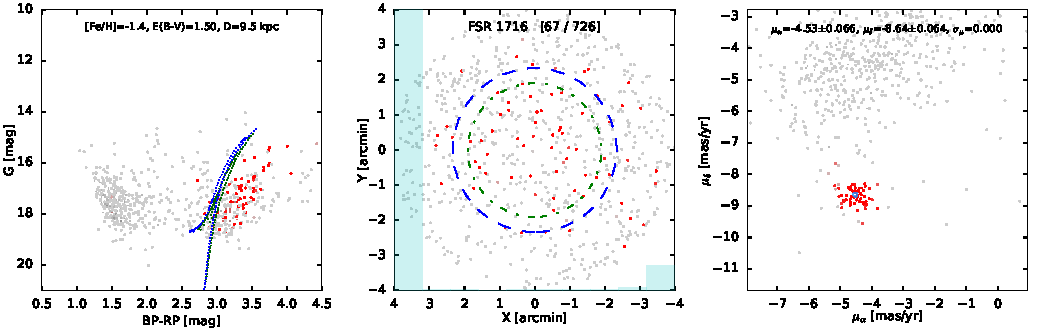
\includegraphics{figs/FSR_1716.pdf}
\end{figure*}

\clearpage\begin{figure*}
\contcaption{}
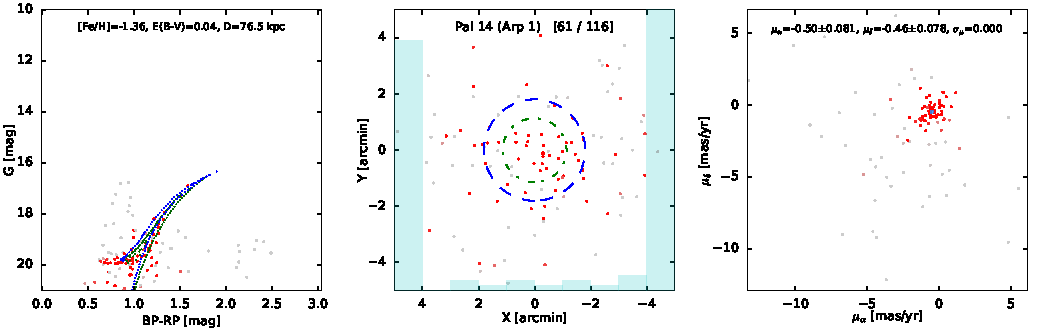
\includegraphics{figs/Pal_14.pdf}
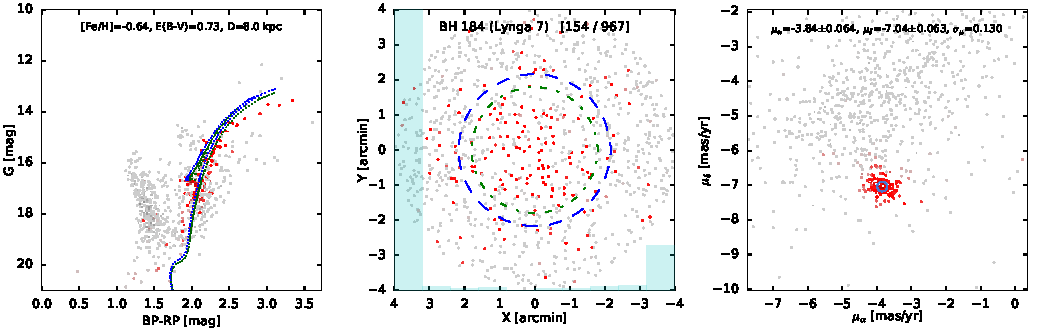
\includegraphics{figs/Lynga_7_BH184.pdf}
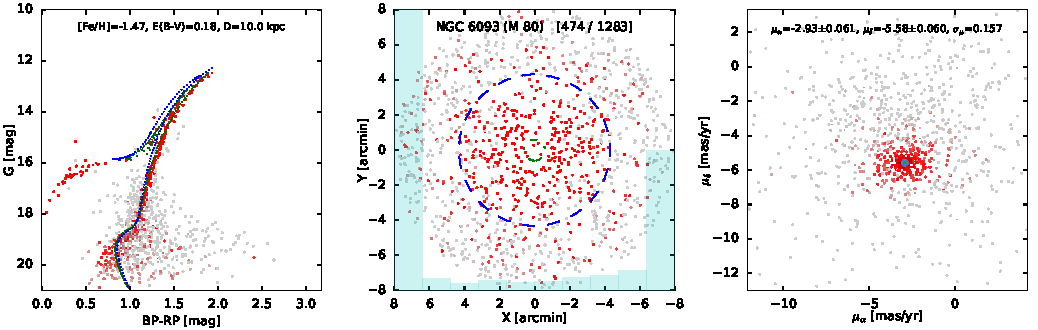
\includegraphics{figs/NGC_6093_M_80.pdf}
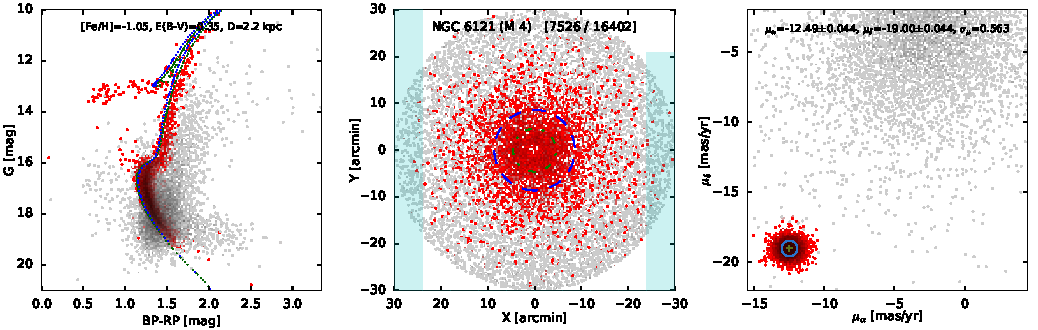
\includegraphics{figs/NGC_6121_M_4.pdf}
\end{figure*}

\clearpage\begin{figure*}
\contcaption{}
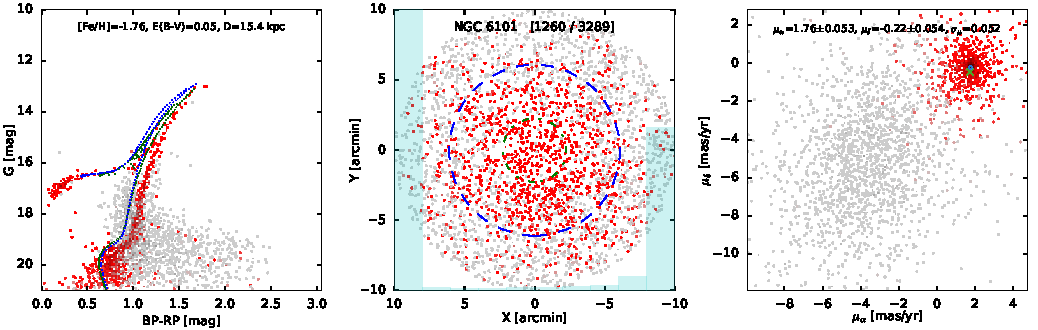
\includegraphics{figs/NGC_6101.pdf}
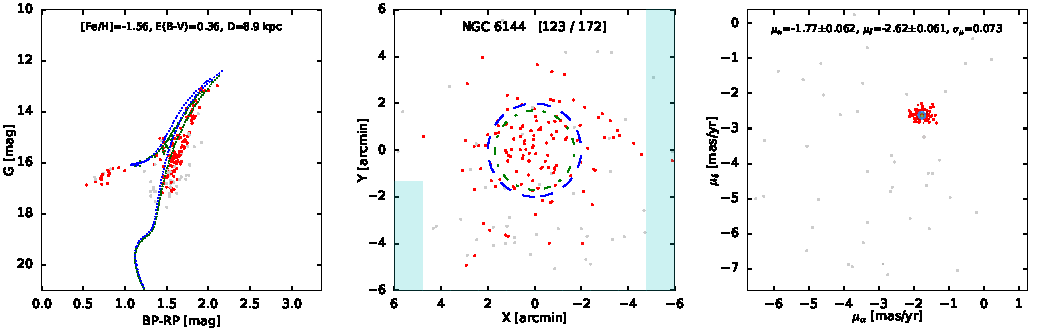
\includegraphics{figs/NGC_6144.pdf}
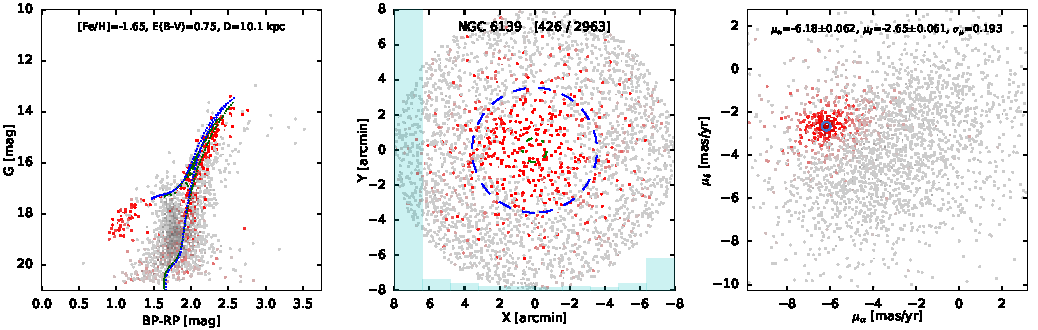
\includegraphics{figs/NGC_6139.pdf}
\includegraphics{figs/Terzan_3.pdf}
\end{figure*}

\clearpage\begin{figure*}
\contcaption{}
\includegraphics{figs/NGC_6171_M107.pdf}
\includegraphics{figs/1636-283_ESO452.pdf}
\includegraphics{figs/NGC_6205_M_13.pdf}
\includegraphics{figs/NGC_6229.pdf}
\end{figure*}

\clearpage\begin{figure*}
\contcaption{}
\includegraphics{figs/NGC_6218_M_12.pdf}
\includegraphics{figs/FSR_1735.pdf}
\includegraphics{figs/NGC_6235.pdf}
\includegraphics{figs/NGC_6254_M_10.pdf}
\end{figure*}

\clearpage\begin{figure*}
\contcaption{}
\includegraphics{figs/NGC_6256.pdf}
\includegraphics{figs/Pal_15.pdf}
\includegraphics{figs/NGC_6266_M_62.pdf}
\includegraphics{figs/NGC_6273_M_19.pdf}
\end{figure*}

\clearpage\begin{figure*}
\contcaption{}
\includegraphics{figs/NGC_6284.pdf}
\includegraphics{figs/NGC_6287.pdf}
\includegraphics{figs/NGC_6293.pdf}
\includegraphics{figs/NGC_6304.pdf}
\end{figure*}

\clearpage\begin{figure*}
\contcaption{}
\includegraphics{figs/NGC_6316.pdf}
\includegraphics{figs/NGC_6341_M_92.pdf}
\includegraphics{figs/NGC_6325.pdf}
\includegraphics{figs/NGC_6333_M_9.pdf}
\end{figure*}

\clearpage\begin{figure*}
\contcaption{}
\includegraphics{figs/NGC_6342.pdf}
\includegraphics{figs/NGC_6356.pdf}
\includegraphics{figs/NGC_6355.pdf}
\includegraphics{figs/NGC_6352.pdf}
\end{figure*}

\clearpage\begin{figure*}
\contcaption{}
\includegraphics{figs/IC_1257.pdf}
\includegraphics{figs/Terzan_2_HP_3.pdf}
\includegraphics{figs/NGC_6366.pdf}
\includegraphics{figs/Terzan_4_HP_4.pdf}
\end{figure*}

\clearpage\begin{figure*}
\contcaption{}
\includegraphics{figs/HP_1_BH_229.pdf}
\includegraphics{figs/NGC_6362.pdf}
\includegraphics{figs/NGC_6380_Ton1.pdf}
\includegraphics{figs/Terzan_1_HP_2.pdf}
\end{figure*}

\clearpage\begin{figure*}
\contcaption{}
\includegraphics{figs/Ton2_Pismis26.pdf}
\includegraphics{figs/NGC_6388.pdf}
\includegraphics{figs/NGC_6402_M_14.pdf}
\includegraphics{figs/NGC_6401.pdf}
\end{figure*}

\clearpage\begin{figure*}
\contcaption{}
\includegraphics{figs/NGC_6397.pdf}
\includegraphics{figs/Pal_6.pdf}
\includegraphics{figs/NGC_6426.pdf}
\includegraphics{figs/Djorg_1.pdf}
\end{figure*}

\clearpage\begin{figure*}
\contcaption{}
\includegraphics{figs/Terzan_5_11.pdf}
\includegraphics{figs/NGC_6440.pdf}
\includegraphics{figs/NGC_6441.pdf}
\includegraphics{figs/Terzan_6_HP_5.pdf}
\end{figure*}

\clearpage\begin{figure*}
\contcaption{}
\includegraphics{figs/NGC_6453.pdf}
\includegraphics{figs/NGC_6496.pdf}
\includegraphics{figs/Terzan_9.pdf}
\includegraphics{figs/Djorg_2_ESO456-.pdf}
\end{figure*}

\clearpage\begin{figure*}
\contcaption{}
\includegraphics{figs/NGC_6517.pdf}
\includegraphics{figs/Terzan_10.pdf}
\includegraphics{figs/NGC_6522.pdf}
\includegraphics{figs/NGC_6535.pdf}
\end{figure*}

\clearpage\begin{figure*}
\contcaption{}
\includegraphics{figs/NGC_6528.pdf}
\includegraphics{figs/NGC_6539.pdf}
\includegraphics{figs/NGC_6540_Djorg.pdf}
\includegraphics{figs/NGC_6544.pdf}
\end{figure*}

\clearpage\begin{figure*}
\contcaption{}
\includegraphics{figs/NGC_6541.pdf}
\includegraphics{figs/ESO-SC06_ESO280.pdf}
\includegraphics{figs/NGC_6553.pdf}
\includegraphics{figs/NGC_6558.pdf}
\end{figure*}

\clearpage\begin{figure*}
\contcaption{}
\includegraphics{figs/IC_1276_Pal_7.pdf}
\includegraphics{figs/Terzan_12.pdf}
\includegraphics{figs/NGC_6569.pdf}
\includegraphics{figs/BH_261_AL_3.pdf}
\end{figure*}

\clearpage\begin{figure*}
\contcaption{}
\includegraphics{figs/NGC_6584.pdf}
\includegraphics{figs/NGC_6624.pdf}
\includegraphics{figs/NGC_6626_M_28.pdf}
\includegraphics{figs/NGC_6638.pdf}
\end{figure*}

\clearpage\begin{figure*}
\contcaption{}
\includegraphics{figs/NGC_6637_M_69.pdf}
\includegraphics{figs/NGC_6642.pdf}
\includegraphics{figs/NGC_6652.pdf}
\includegraphics{figs/NGC_6656_M_22.pdf}
\end{figure*}

\clearpage\begin{figure*}
\contcaption{}
\includegraphics{figs/Pal_8.pdf}
\includegraphics{figs/NGC_6681_M_70.pdf}
\includegraphics{figs/NGC_6712.pdf}
\includegraphics{figs/NGC_6715_M_54.pdf}
\end{figure*}

\clearpage\begin{figure*}
\contcaption{}
\includegraphics{figs/NGC_6717_Pal9.pdf}
\includegraphics{figs/NGC_6723.pdf}
\includegraphics{figs/NGC_6749.pdf}
\includegraphics{figs/NGC_6752.pdf}
\end{figure*}

\clearpage\begin{figure*}
\contcaption{}
\includegraphics{figs/NGC_6760.pdf}
\includegraphics{figs/NGC_6779_M_56.pdf}
\includegraphics{figs/Terzan_7.pdf}
\includegraphics{figs/Pal_10.pdf}
\end{figure*}

\clearpage\begin{figure*}
\contcaption{}
\includegraphics{figs/Arp_2.pdf}
\includegraphics{figs/NGC_6809_M_55.pdf}
\includegraphics{figs/Terzan_8.pdf}
\includegraphics{figs/Pal_11.pdf}
\end{figure*}

\clearpage\begin{figure*}
\contcaption{}
\includegraphics{figs/NGC_6838_M_71.pdf}
\includegraphics{figs/NGC_6864_M_75.pdf}
\includegraphics{figs/NGC_6934.pdf}
\includegraphics{figs/NGC_6981_M_72.pdf}
\end{figure*}

\clearpage\begin{figure*}
\contcaption{}
\includegraphics{figs/NGC_7006.pdf}
\includegraphics{figs/NGC_7078_M_15.pdf}
\includegraphics{figs/NGC_7089_M_2.pdf}
\includegraphics{figs/NGC_7099_M_30.pdf}
\end{figure*}

\clearpage\begin{figure*}
\contcaption{}
\includegraphics{figs/Pal_12.pdf}
\includegraphics{figs/Pal_13.pdf}
\includegraphics{figs/NGC_7492.pdf}
\end{figure*}

\clearpage
\begin{thebibliography}{}

\bibitem[Babusiaux et al.(2018)]{Babusiaux2018}
Babusiaux C., van Leeuwen F., Barstow M., et al. (\Gaia Collaboration), 2018, A\&A, 616, 10
%Gaia HR diagram and extinction coefficients

\bibitem[Baumgardt et al.(2019)]{Baumgardt2019}
Baumgardt H., Hilker M., Sollima A., Bellini A., 2019, MNRAS, 482, 5138
%GC catalog with Gaia PM for internal kinematics

\bibitem[Bressan et al.(2012)]{Bressan2012}
Bressan A., Marigo P., Girardi L., et al., 2012, MNRAS, 427, 127
%PARSEC isochrones

\bibitem[Choi et al.(2016)]{Choi2016}
Choi J., Dotter A., Conroy C., et al., 2016, ApJ, 823, 102
%MIST isochrones

\bibitem[Helmi et al.(2018)]{Helmi2018}
Helmi A., van Leeuwen F., McMillan P., et al. (\Gaia Collaboration), 2018a, A\&A, 616, 12 (H18)
%Gaia DR2 for MW globular clusters

\end{thebibliography}

\end{document}